% Needed packages
\documentclass[a4paper, 10pt, english, onecolumn]{article}
\usepackage[english]{babel}
\usepackage[cm]{fullpage}
\usepackage{cite}
\usepackage{anysize}
\usepackage{setspace}
%\usepackage[compact]{titlesec}
\usepackage{graphicx}
\usepackage{stfloats}
\usepackage{listings}
\usepackage{hyperref}

\usepackage{amssymb,amsmath}
\usepackage{algorithmicx}
%\usepackage{algorithmic}
\usepackage{algorithm}
\usepackage[noend]{algpseudocode}

% for coloring individual cells in a table
\usepackage[table]{xcolor}
%\usepackage{pgfgantt}

%\newcommand{\keywords}[1]{\par\noindent 
%{\bf Keywords\/}. #1}

% Margins & Headers
\marginsize{2.5cm}{2.5cm}{3.0cm}{2.0cm}
\columnsep 0.4in
\footskip 0.4in 
\usepackage{changepage}

% E-mail formatting
\usepackage{color,hyperref}
    \catcode`\_=11\relax
    \newcommand\email[1]{\_email #1\q_nil}
    \def\_email#1@#2\q_nil{
      \href{mailto:#1@#2}{{\emailfont #1\emailampersat #2}}
    }
    \newcommand\emailfont{\sffamily}
    \newcommand\emailampersat{{\color{red}\small@}}
    \catcode`\_=8\relax 
	
% List modifications
\newenvironment{packed_item}{
\begin{itemize}
  \setlength{\itemsep}{1pt}
  \setlength{\parskip}{0pt}
  \setlength{\parsep}{0pt}
}{\end{itemize}}

\newenvironment{packed_enum}{
\begin{enumerate}
  \setlength{\itemsep}{1pt}
  \setlength{\parskip}{0pt}
  \setlength{\parsep}{0pt}
}{\end{enumerate}}

% ### Mathematics ###
\newcommand{\bpm}{\begin{pmatrix}}
\newcommand{\epm}{\end{pmatrix}}

\newcommand{\bbm}{\begin{bmatrix}}
\newcommand{\ebm}{\end{bmatrix}}

\newcommand{\bsm}{\bigl( \begin{smallmatrix}}
\newcommand{\esm}{ \end{smallmatrix} \bigl)} 

\newcommand{\mbf}{\mathbf}

% ### Matrices and Vectors ###
\newcommand{\mtx}[1]{\ensuremath{\boldsymbol{#1}}}
\newcommand*\Let[2]{\State #1 $\gets$ #2}

% ### Sets ###
\newcommand{\set}[1]{\ensuremath{\mathcal{#1}}}

% ### Other ###

\newcommand{\transpose}{^{T}}
\newcommand{\inv}{^{-1}}
\newcommand{\pseudoinv}{^{+}}

% ### Hyphenation ###
\hyphenation{a-na-ly-sis}

% ### dots at the end of arrows and lines ###

\def \orightarrow {\circ\hspace{-0.42em}\rightarrow}
\def \oleftarrow {\leftarrow\hspace{-0.42em}\circ}
\def \orightline {\circ\hspace{-0.16em}-}
\def \oleftline {-\hspace{-0.16em}\circ}
\def \oline {\circ\hspace{-0.38em}-\hspace{-0.2em}\circ}
\def \srightarrow {\text{\textasteriskcentered}\hspace{-0.62em}\rightarrow}
\def \sleftarrow {\leftarrow\hspace{-0.62em}\text{\textasteriskcentered}}
\def \srightline {\text{\textasteriskcentered}\hspace{-0.16em}-}
\def \sleftline {-\hspace{-0.40em}\text{\textasteriskcentered}}
\def \sline {\text{\textasteriskcentered}\hspace{-0.38em}-\hspace{-0.4em}\text{\textasteriskcentered}}
\def \soline {\text{\textasteriskcentered}\hspace{-0.16em}-\hspace{-0.4em}\circ}
\def \osline {\circ\hspace{-0.38em}-\hspace{-0.16em}\text{\textasteriskcentered}}

% ############## End Macros ##############

% ### Section Formatting ###
\usepackage[compact]{titlesec}
\titlespacing*{\section}{4pt}{*0}{4pt}

% ### Paragraph Formatting ###
\makeatletter
\renewcommand{\paragraph}{%
  \@startsection{paragraph}{4}%
  {\z@}{0.5ex \@plus 1ex \@minus .2ex}{-1em}%
  {\normalfont\normalsize\bfseries}%
}
\makeatother

% Title
\title{\fontfamily{phv}\selectfont{Causal Discovery methods for Effective Connectivity in Human Brains}}
\author{
  \textbf{R. Janssen} - \href{mailto:ramon.janssen@student.ru.nl}{ramon.janssen@student.ru.nl} \\
  \textbf{T. de Ruijter} - \href{mailto:t.deruijter@student.ru.nl}{t.deruijter@student.ru.nl}\\
%  \textbf{T. Claassen} - \href{mailto:tomc@cs.ru.nl}{tomc@cs.ru.nl}\\
%  \textbf{M. Hinne} - \href{mailto:mhinne@cs.ru.nl}{mhinne@cs.ru.nl}
}

\date{\fontfamily{ptm}\selectfont{\small{\bfseries{\today - Radboud
Universiteit Nijmegen}}}\\[0.5cm]\rule{\linewidth}{0.3mm}}

\begin{document}

\maketitle

\setlength{\parindent}{0.0cm}
\setlength{\parskip}{3mm plus2mm minus1.5mm}

\begin{abstract}
% TODO: first state what you try to do, then how you did it, then what it brought you
%In this work we applied PC algorithm on resting-state data of healthy human subjects.
%Additionally we propose a variant of PC algorithm that poses weaker assumptions on the model, better fitting the underlying model.
%We find that detecting structure homological areas in the brain works better with PC algorithm than most conventional diffusion weighted imaging techniques.
%In the area of directionality and causality, more research is needed.
\end{abstract}
\section{Introduction}
\subsection{Subject introduction}
%Effective connectivity resting state analysis in human brains
%Resting state
%Brains are networks; apply graphical models and causal discovery

\subsection{ Motivation for research}
%Better understanding of brains
%Relatively new field - not yet an established analysis method
%Existing problems with current methods and applications, specifically [Tom: mention all, or just the relevant problems?]
%- Model selection
%- Indirect measurements
%- Modelling causal structure across individuals (varying responses to same stimuli)
%- Distinct but overlapping ROIs
%- Varying Haemodynamic response (HRF)
%Find shortcomings of PC and improve it (EMS-PC)

\subsection{Problem statement}
%See whether applying causal methods (PC and EMS-PC) can help bring new insights and whether we can find evidence for the existence of causal patterns on a whole brain level.

\subsection{Previous research}
%[Tom: we did not explicitly have this paragraph, so this is additional effort]
%[Ramon]: Lijkt me vergelijkbaar met de verwijzingen naar literatuur die we al hebben? Met wat extra referenties naar wat Max zei: temporele methodes zijn onbetrouwbaar, dat hebben wij niet
%[Ramon]: even een goede balans zoeken tussen dit en "Existing problems" in motivation

\subsection{Research goal}
%How does the standard causal discovery method PC Algorithm behave regarding the aforementioned problems when applied to resting-state functional time-series data?
%- Can we overcome the consistency problems of PC algorithm applied on resting-state functional data?
%- Does the PC algorithm applied on resting-state functional data provide consistent, specific and anatomically plausible connectivity?
%- How does functional connectivity found by the first part of PC relate to other structural / functional methods applied on the same resting-state functional data regarding the aforementioned problems?
%
%How does the performance of EMS-PC relate to PC regarding the aforementioned problems when applied to the same resting-state functional time-series data?
%- When would EMS-PC perform better than PC algorithm regarding directionality results?
%- Is EMS-PC more consistent in its results within a single subject than PC algorithm on resting-state functional data, regarding the multiple separating set addition and the explicit v-structure test?
%- Can we find unfaithfulness within our model without additional independence tests?


\subsection{Relevance of research}
%If HRF can be avoided, causal patterns can be established with greater reliability
%Insight and diagnostics in neuro-degenerative diseases
%Any found evidence of causal patterns can give an impulse to further research
%[Ramon: is dit niet al duidelijk uit motivation? Lijkt me dubbelop]

\section{Background}
\subsection{Types of brain connectivity}% [optional] [Ramon: lijkt me wel belangijk, geeft ook het belang aan van richting zoeken, hoeft niet lang]
%Functional
%Structural
%Effective

\subsection{Causal discovery theory}
%Causal Markov Condition
%Causal faithfulness
%d-separation
%V-structure
%Causal sufficiency
%Latent variables

\subsection{PC algorithm}
%Algorithm, assumptions and explanation
\paragraph{Description}
The PC algorithm is a so-called constraint based method, where solutions are found by incrementally leaving out or adding parts that do not violate a set of constraints.
Starting from a fully connected undirected graph, the PC algorithm forms structure by cutting away edges between conditionally independent variables.
In the second step, orientation rules are applied based on found separating sets and structure.
The original PC algorithm assumes causal sufficiency, excluding the existence of common confounders between nodes.
This seems unwanted when handling brain data, where one would expect a large amount of latent processes.
Also measuring methods are not yet advanced enough to measure detailed neuronal processing of the brain, thus skipping over details.
In the perspective of causal inference, these missing areas can also appear as confounders.
For the following experiments we have used the causal insufficient version of PC algorithm, modified to handle latent variable as described by Spirtes, Glymour and Scheines \cite[p.165-167]{spirtes2000}.
From now on, we will refer to this algorithm as \textit{standard PC}.
Pseudocode for this method is shown in algorithm~\ref{alg:pc_alg}.

\begin{algorithm}
\caption{Standard PC algorithm}
\begin{spacing}{1.1}
\begin{algorithmic}[1]
\Function{PC}{$data$}
\State connect all pairs of point in undirected graph $G$. \label{alg:pc_alg:p1_start}
                                                                                                                                    \Comment{Structural Part} 
\State $n \gets 0$
\While{there are connected pairs ($X$, $Y$) such that $n < |\operatorname{Adjacencies}(X)\setminus\{Y\}| $}
  \ForAll{such connected pairs ($X$, $Y$)}
    \ForAll{subsets $S$ of $\operatorname{Adjacencies(X)}$ for which $|S| = n$}
      \If{$X$ and $Y$ are independent given $S$}
        \State remove edge $X - Y$ from G
        \State record $S$ as separating set of ($X, Y$)
        \State continue with the next pair ($X$, $Y$) \label{alg:pc_alg:next_pair}
      \EndIf
    \EndFor
  \EndFor
  \State $n \gets n+1$ \label{alg:pc_alg:p1_end}
\EndWhile
\\
\State $\text{PDAG} \gets G\text{, with all connections replaced by }\oline$ \label{alg:pc_alg:p2_start}
                                                                                                                                    \Comment{Directional Part}
\ForAll{unshielded triples $\left <X, Y,Z \right> $ in $G$ }
                                                                                                                                    \Comment{Find V-structures}
  \If{$Y$ is not in the separating set of $X$ and $Z$} \label{alg:pc_alg:v_struct}
    \State Orient $X \sline Y \sline Z$ as $X \srightarrow Y \sleftarrow Z$ in $\text{PDAG}$
  \EndIf
\EndFor
\While{Edges can still be oriented}
                                                                                                                                    \Comment{Additional orientations}
  \If{there is an edge $X \sline Y$, and there is a directed path from $X$ to $Y$}
    \State orient $X \sline Y$ as $X \rightarrow Y$
  \EndIf
  \If{there are edges $X \srightarrow Y$ and $Y \sleftline Z$, the latter is not an edge $Y \sleftarrow Z$}
    \If{$X$ and $Z$ are not connected}
      \State orient $Y \sline Z$ as $Y \rightarrow Z$
    \EndIf
  \EndIf
\EndWhile
\State \Return $G$ and the separating sets \label{alg:pc_alg:p2_end}
\EndFunction
\end{algorithmic}
\end{spacing}
\label{alg:pc_alg}
\end{algorithm}

Starting from a fully connected graph, standard PC finds a minimal separating set for every pair of non-adjacent nodes $X$ and $Y$.
These are lines~\ref{alg:pc_alg:p1_start} to \ref{alg:pc_alg:p1_end} in the pseudocode.
The independence of $X$ and $Y$ is tested given a subset of neighbours of $X$ or $Y$ using a statistical independence test such as the Chi-square or Fisher-Z independence tests. %TODO: Add citation to these methods.
If such an independence is found, this subset is a separating set of $X$ and $Y$ and they are not connected.
If no such set can be found, the variables are assumed to be dependent and thus remain connected.
To find a minimal separating set, all subsets of neighbours are traversed in order of size; the first separating set which is found, is the minimal one.

Next, PC algorithm attempts to orient these edges.
These are lines~\ref{alg:pc_alg:p2_start} to \ref{alg:pc_alg:p2_end} in the pseudocode.
The 'o' mark represents that it is unknown what orientation the specific edge should have thus representing an entire Markov class of solutions rather than a specific instance.
Like Spirtes et al, we use a star-symbol at the end of an edge to denote that any mark may be present: an arrowhead, an "o" or an empty mark.
When an edge is oriented as an edge with a star, this denotes that this end is not changed.
The first of the directionality rules attempts to orient unshielded triples.
For a triple $\left < X,Y,Z, \right>$ to be oriented, $X$ and $Z$ should have a separating set $S$ not containing $Y$.
If so, the triple is marked a V-structure.
After all V-structures have been found, the other rules are applied in no particular order.
These rules are based on already found directionality.

\paragraph{Run-time performance}
The PC algorithm run-time is in the order of the amount of dependency tests to be performed and thus it has a worst-case runtime complexity exponential in the maximal branching degree present in the graph.
However, this worst-case scenario only happens when no edges can be removed; all subsets of the complete set of nodes have to be used to test d-separation of every pair of nodes.
For a sparse graph, many edges may be removed for small separating sets, and this enables the standard PC algorithm to often run fast in practice perform well on hundreds of variables. % TODO: add citation to example publication. Peter Lucas maybe or examples in the sprites book?

\paragraph{Shortcomings}
Although PC is proven correct, the version provided above as standard PC is not.
It is also not complete.
There is additional the number of possible graphs in the returned Markov class increasing exponentially with the amount of variables in the provided data, thus not always providing ample information.
Also, standard PC is dependent on the order in which these variables are presented, as this is the same order in which edges between pairs of these variables are considered for removal\cite[p.88]{spirtes2000}.

In practice, the lack of full correctness and completeness are of little concern as these involve only very specific and little occurring connectivity patterns\cite[p.127-130]{spirtes2000}.
% TODO: Paragraph seems incomplete and some sentences are weird.

\paragraph{Conservative PC extension}
The V-structure rule in PC algorithm orients unshielded triples based on a single separating set. 
Simply put, it is assumed the single found separating set is enough to show conditional independence. 
Ramsey et al. \cite{ramsey2012} introduce a weaker but still sufficient assumption for finding V-structures.
Through this weaker but still adjacency-faithful assumption, the method is more cautious than PC algorithm in drawing unambiguous conclusions on causal orientations.
That is why this method is named Conservative PC (CPC).
The resulting algorithmic changes provide better results and is able to mark incorrectly unshielded triples as unfaithful.
Sadly, CPC requires a significant amount of additional conditional independence tests, exponential in the largest branching degree of the tested structure.
Although the weaker assumptions made with conservative PC might be useful for this research, the run-time performance is not good enough to apply it on our dataset.

\section{Methods}% (our contributions)
Standard PC provides a good starting point for an exploratory point of view in causal discovery.
Already with simple and small adjustments to standard PC with little increment in computational cost, standard PC can be made more reliable.
In the rest of this section we describe our additions to this method, as well as an experimental setup

\subsection{Improvements to PC}
%Multiple separating sets and why it should be better / not worse (correctness, runtime)
\paragraph{Multiple Separating Sets}
As can be seen in the result in the next section, standard PC is a bit hasty in assigning v-structures, resulting in much unnecessary and perhaps unfaithful directionality.
The idea of CPC, to rely less on graph faithfulness than standard PC is potential as less erroneous arrows are assigned in theory.
Instead of doing additional tests as described in CPC, one could attempt to determine causal unfaithfulness with less dependency tests.
An adaptation to PC algorithm that would not increase the order of complexity is once a separating set is found to test all other vertex subsets of the same order as well.
This finds all separating sets of the lowest order without increasing complexity.
Orienting an unshielded triple $\left<A,B,C\right>$ requires $B$ not to occur in any separating set of $(A,C)$.
By having more than one separating set, this constraint is strengthened in case of noisy data.
% Unfaithfulness test
One could use these additional separating sets to test oriented unshielded triples for unfaithfulness, similar to CPC.
Apart from serving as a sanity check, this could serve as the basis of a repair algorithm for errors made by PC.

% Explicit test
\paragraph{Explicit V-structure test}
A more \textit{explicit} way to decrease faulty orientation of an unshielded triple $\left<A,B,C\right>$ is to check whether adding $B$ to a separating set of $(A,C)$ makes the pair conditionally dependent.
If so, the graph might become more faithful to its modeled distribution; If standard PC might orient a V-structure, whereas this condition does not hold, then the concluded V-structure might be erroneous.
For faithful graphs, this extra condition should not change the result, as it will always hold.

%EMS-PC extension (no pseudo-code, but additions regarding standard PC)
\paragraph{EMS-PC}
We have combined the above ideas - multiple separating sets, unfaithfulness check and explicit orientation check - into an adaptation of PC, which we refer to as Explicit Multiple Separating Set PC (EMS-PC).
These three changes have been made in this adaption with respect to standard PC as described in algorithm~\ref{alg:pc_alg}.
At line~\ref{alg:pc_alg:next_pair}, the search for separating sets for $X$ and $Y$ stops when a separating set is found; instead, EMS continues the search for more separating sets of the same order.
All of these separating sets are recorded.

Also, the condition on line~\ref{alg:pc_alg:v_struct} to orient $X - Y - Z$ according to the V-structure-rule has been made more strict.
As multiple separating sets have been found instead of only one, it needs to be checked whether $Y$ is in not in \emph{any} of those sets before the V-structure can be oriented.
In addition to this original condition, $X$ and $Z$ are \textit{explicitly} tested for \textit{d}-separation given $\{Y\}$.
If they are found to be conditionally \textit{dependent}, the triple is oriented as as $X \srightarrow Y \sleftarrow Z$.
Otherwise it is not oriented.

Given the found separating sets, it is possible to test whether these sets provide a consistent answer to the question whether the unshielded triple $\left<X,Y,Z\right>$ is \textit{d}-separated by $Y$.
It should be the case that $Y$ occurs in all found separating sets.
If this is not the case, the triple is marked as unfaithful.
This can be used as a diagnostic to judge initial reliability of results without almost any additional computational cost.
The marked triples could be coloured differently in the resulting 
The downside of this additional check is results are merely used as a diagnostic and thus the unshielded triple is oriented in a v-structure nevertheless.
It is also not a complete check as this would require as many tests as in CPC and thus no positive conclusions can be drawn from it.
Also if an unfaithful triple is detected, the impact on the final output is unclear as errors might have cascaded into further orientation steps.

\subsection{Experimental validation}
\paragraph{Experimental pipeline}\label{sec:pipeline}
%- What type of data is needed
PC algorithm requires observational data where each instance is a vector of single observations per variable.
We can model functional resting-state time-series as coming from some stable underlying mechanism that is largely time-independent.
Resting-state data can be intuitively thought of being more time independent than task-influenced data due to the emergent character of activity pattens that occur when in resting-state.
Nevertheless it is most likely not a fully correct modelling assumption, though enables straightforward application of standard and EMS-PC to functional data without the problem of HRF.

% Application to data
We applied standard PC and EMS-PC on functional resting-state time-series data of six healthy individuals, also previously used by Hinne et al\cite{hinne2013}.
1030 volumes were obtained per subject.
After preprocessing the fMRI data was parcellated according to the Automated Anatomical Labeling (AAL) atlas in 116 regions of interest.
The exact procedure of subject acquisition, used scanner properties and parameters and data preprocessing is provided in appendix~\ref{sec:data}.
We use Fisher's z-test for conditional independence to match the continuous nature of the data.

% Implementation
We have implemented standard PC and EMS-PC in Matlab using statistical tests and ideas from the Bayesian Network Toolbox for Matlab.\footnote{Bayesian Network Toolbox for Matlab: https://github.com/bayesnet/bnt}
This toolbox also includes an implementation for standard PC, however to gain better insight in the workings and to have greater flexibility in application, we have implemented standard PC separately.
The Matlab scripts used for the results are made freely available online.\footnote{Matlab implementation of EMS-PC: https://github.com/tomderuijter/EMS-PC}

% Pipeline
For all experiments we first apply part 1 of standard PC and EMS-PC on the data.
This results in a graph describing undirected functional connections between regions.
For structure only the first found separating set is relevant, thus EMS-PC and standard PC return identical graph structure.
This structure is then oriented with part 2 of standard PC and EMS-PC given earlier found separating sets.
This procedure yields different orientations in theory.

% Stability selection
Standard PC depends on the ordering of variables in the provided data\cite[p.120-122]{spirtes2000}.
It is therefore questionable whether strong conclusions about individual edges can be drawn from the output, as such an edge might not have appeared if the input was ordered differently.
To correct for this in results, we have randomly permuted our data for a large amount of iterations and counted the frequencies of occurring edges.
This is in accordance with the stability selection method for graphs as described by Meinshausen and B{\"u}hlmann\cite{meinshausen2010}.

% Parameter selection
Due to the lack of a baseline to compare results with, dependency thresholds were chosen by hand.
All experiments listed here were run with an alpha value of 0.01 for the independence test.
The number of random permutations was set on 1000 per subject, which was found to be enough to determine statistical significance for 99\% of the found edges with a binomial statistical test.

% Structural and Directional Consistency
% DWI Comparison
We obtained structure and causal graphs for each subject with the previous procedure.
For each graph, we express the level of consistency of an edge in the frequency of occurrence of that type of edge over all permutations.
The frequency ratio per is then used to create the whole brain image for structure and directionality.
We compared the generated functional graph with the Bayesian inference approach on finding structural connectivity from Diffusion Weighted Imaging (DWI) proposed by Hinne et al.\cite{hinne2013} on the same data using edge consistency.

%Markov equivalence class size and asymmetry
Since standard PC and EMS-PC return Markov equivalence classes, we record the size of the solution space per subject.
Different permutations of nodes may yield different directionality for the same edge, including bi-directional relationships.
Of specific interest are consistent non-symmetrical orientations, as one-directional arrows imply a high-confidence causal relation.
Bi-directional edges imply an unseen common confounder.
We obtain uni-directional edges by subtracting the symmetrical bi-directional components from the causal graph.

% Multi-subject experiments
To aggregate results over multiple subjects, we sum frequencies per found edge type for structure and directionality to obtain consistency of edges and directionality.
We expected brain functioning to not completely differ between subjects.

% EMS-PC
For results on EMS-PC, we record the size of the separating sets found per edge as well as the amount of unfaithful marked v-structures.

% Comparison standard PC and EMS-PC
We compare standard PC and EMS-PC on their causal graph.
As EMS-PC is more constrained in concluding directionality, it may find less erroneous edges than standard PC.
As we cannot verify this directly, we compare the total count, consistency and standard-deviation of one-directional arrows.
%- Run-time of methods and comparison between run-times
We also compare run-time per iteration between both.

\section{Results}\label{sec:results}
Due to the size of the resulting graphs, we represent them in the form of connectivity matrices for convenience.
A connection from region $n$ to region $m$ is represented by point $(n,m)$ in the matrix.
Higher values represent higher frequencies of a connection over all permutations.
In all matrices, indices 1-45 represent the brain regions of the left hemisphere, indices 45-90 represent the right hemisphere, and indices 91-116 represent regions in the cerebellum.
% For clarification, these are also plotted separately.

\subsection{Structural graph}
%- Measuring whole-brain structural and directional consistency of PC - frequency of occurrences within subjects
%Applying the standard PC algorithm yields an undirected graph, in which each edge has a certainty.
%This is done both per subject, and as an avarage over all subjects.
%We compared the generated structure with a Bayesian inference approach on finding structural connectivity from diffusion weighted imaging, as described in Hinne et al.\cite{hinne2013}.
Modified PC and EMS-PC do not differ in finding the structure.
As edges found with the structural part of PC are undirected, the found matrices are symmetrical.
The results are presented per subject in figure~\ref{} and as an avarage across all subjects in figure~\ref{fig:struct_avg}. %TODO: figure fixen per subjects
For comparison, the structural connectivity as found by Hinne et al.\cite{hinne2013} are also show. 

\begin{figure}[h!]
  \centering
  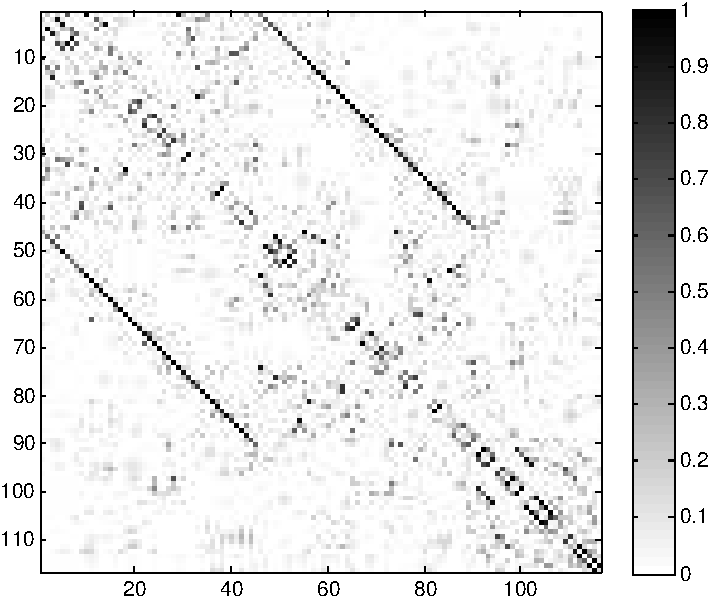
\includegraphics[width=0.5\textwidth]{images/struct_full}
  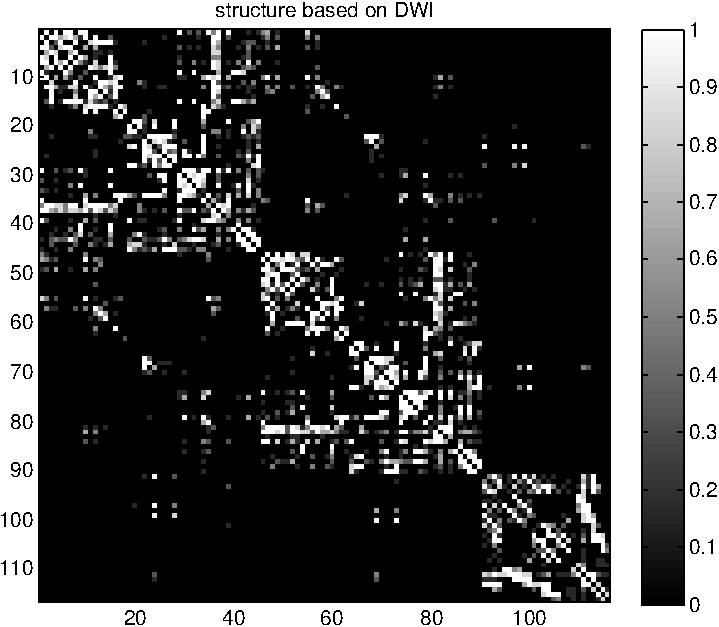
\includegraphics[width=0.5\textwidth]{images/structure_max}
  \caption{The avarage structure of all subjects. The structure on the left is found with the PC-algorithm, and the structure on the right is found with DWI-measurements by Hinne et al. Note that these matrices are subdivided into blocks corresponding with the subdivision of indices as described in section~\ref{sec:results}. The two diagonal lines represent connections between the two hemispheres.}
\label{fig:struct_avg}
\end{figure}

\subsection{Causal graph}
This structural graph has been used as a basis for a directed graph, for both standard PC and EMS-PC.
The results for standard PC are shown per subject in Figure~\ref{} and in as an avarage across subjects in figure~\ref{fig:pdag_avg_mod}.
Additionally, a histogram showing the frequencies of the values in the avarage matrix is presented in figure~\ref{}.
Although many arrowheads are found with probabilities above 0.9, the graph looks strongly symmetric.
In terms of causality, this means that many latent sources are still present and causal relations between the measured brain regions themselves are not clearly visible.

The results for EMS-PC are presented in a similar way. The results per subjects are shown in figure~\ref{} and the avarage across subjects in figure~\ref{fig:pdag_avg_ems}. A histogram of the average is presented in figure~\ref{}. Again, the image looks strongly symmetric.

\begin{figure}[h!]
  \centering
  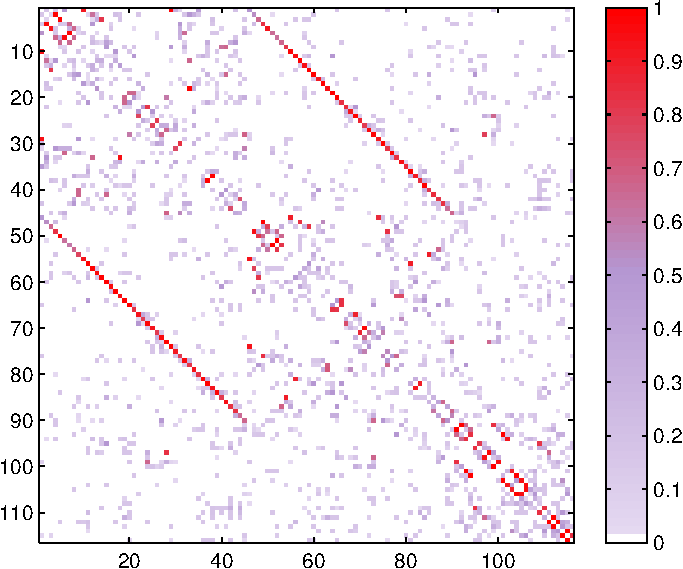
\includegraphics{images/pdag_avg_colored_mod}
  \caption{The PDAG found with standard PC, in which a high value denotes a high certainty of an arrowhead. The avarage of all six subjects is taken.}
  \label{fig:pdag_avg_mod}
\end{figure}

\begin{figure}[h!]
  \centering
  \includegraphics{images/PDAG_avg_colored_expl}
  \caption{The PDAG found with EMS-PC, in which a high value denotes a high certainty of an arrowhead. The avarage of all six subjects is taken.}
  \label{fig:pdag_avg_ems}
\end{figure}

Another representation of this data has been used to emphasise the asymmetric parts of Figures ~\ref{fig:pdag_avg_mod} and ~\ref{fig:pdag_avg_ems}.
To achieve this, the absolute difference between these matrices and their transpose has been calculated, lifting out those points for which there is an arrow in one direction, but not in the opposite direction.
These resulting antisymmetric matrices are presented in Figures ~\ref{fig:pdag_avg_antisymmetric_mod} and ~\ref{fig:pdag_avg_antisymmetric_ems}.

\begin{figure}[h!]
  \centering
  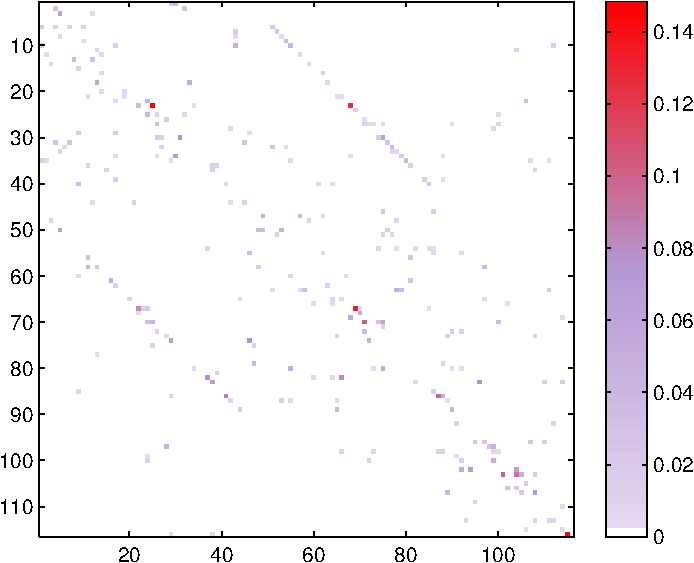
\includegraphics{images/arrowheads_avg_mod}
  \caption{The asymmetric arrowheads of the PDAG found with standard PC, in which a high value denotes a high certainty of an one-directional arrow. The average of all six subjects is taken.}
  \label{fig:pdag_avg_antisymmetric_mod}
\end{figure}

\begin{figure}[h!]
  \centering
  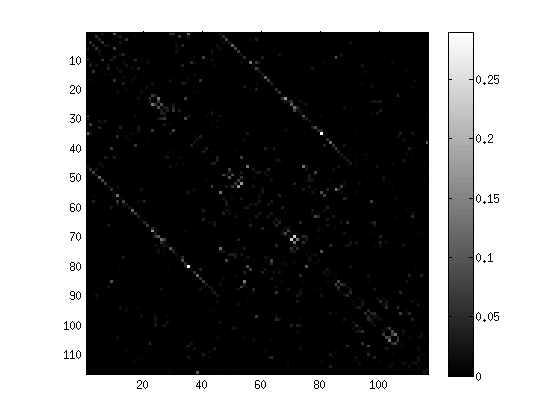
\includegraphics{images/PDAG_avg_antisymmetric_expl}
  \caption{The assymetric parts of the PDAG found with EMS-PC, in which a high value denotes a high certainty of an one-directional arrow. The avarage of all six subjects is taken.}
  \label{fig:pdag_avg_antisymmetric_ems}
\end{figure}

%Again, a certainty of each individual arrowhead may be found by applying stability selection.
%- Markov equivalence class size (nr. of latent variables / bidirectional arrows) within subjects
%Different permutations of nodes may yield different directionalities for the same edge, and bi-directional arrows may be found.
%Of specific interest here are consistent non-symmetrical orientations, as one-directional arrows imlpy a causal relation.
%Edges of two arrowhead imply a common confounder.
%- Markov class Asymmetry and certain asymmetry within subjects
%- Consistency of structure across subjects when aggregating results (averaging and frequency of occurences)
%The results will again be analyses per subject, and as an avarage over all subjects; Causal relations appearing in specific subjects will, or in general.
%- Consistency of directionality across subjects when aggregating results
%The functioning of the brain will not completely differ between different subjects and therefore some consistency across subjects is expected.
%Consistency between the two hemispheres is also expected, as they are anatomically symmetrical.

%\paragraph{EMS-PC}   Er werd veel herhaald t.o.v. standard PC, dus ik heb ze samen genomen. amount of sepsets en faithfulness is niet dubbel, maar hebben we deze resultaten opgeslagen en kunnen we er iets nuttigs over zeggen?
%- Measuring whole-brain structural and directional consistency of EMS-PC
%- Markov equivalence class size (nr. of latent variables / bidirectional arrows) within subjects
%- Markov class Asymmetry and certain asymmetry within subjects
%- Amount of separating sets found
%- Unfaithfulness check with and without additional separating sets

%\paragraph{Comparison between standard PC and EMS-PC}
%- Comparison of directionality between standard PC and EMS-PC on consistency of results within subjects
%As EMS-PC is more constrained in concluding directionality, it may find less erroneous arrows than standard PC.
%To verify this, the number and consistency of one-directional arrows is compared.
%- Comparison of ... of results across subjects
%Again, this is both done per-subject and on the average across subjects.
%- Run-time of methods and comparison between run-times
%The run-time of both methods will be compared.
%- Comparison of structure (functional connectivity) of PC (both. they're identical in structure) with DWI results by Max et al. -> verplaatst naar het stukje aan het begin, over structure PC

%Answer all the questions as mentioned in methods, in the same order
%No aggregation over direction, motivate this

\section{Discussion}
%Good consistency of structure within and between subjects

%HRF

% TODO: Maak duidelijk welke aannames gedaan worden in welke PC variant en welke aannames verzwakt zouden kunnen worden.

% Quick run-time
For PC as well as standard PC we were able to run hundreds of iterations on 116 variables in a matter of hours per subject.
Iterations can also be run in parallel.
Further speed increments can be achieved by coding the algorithm in a low overhead language.

%Comparison with DWI inter-hemisphere connection
Standard PC and particularly the first, structural part, definitely has similarity with respect to existing methods based on DWI.
This is not completely surprising as standard PC yields a functional network and DWI based methods yield anatomical structural networks, two network types which are tightly related.
A less apparent observation is the clear presence of correlation between homologous area's in the functional network, which lacks in the structural network as found with DWI.
An explanation to this difference might be that these correlations respond to the long white-matter tracts connecting the two hemispheres through the corpus-callosum.
It is known that DWI has difficulty in measuring such long tracts, while the presence of correlation between two connected ends cannot be argued against.
As such, statistical baed causal discovery methods contribute additional information to finding structural connectivity.

% Comparison Markov class standard PC and EMS-PC
Both standard PC and EMS-PC find many bi-directional arrows, with some one-directional arrows.
% TODO: find out how large these groups are.

%Poor consistency of directionality between subjects
There is some significant and consistent directionality within each of the subjects.
However the variance of this directionality between subjects is so high, there is no significant consistent one-directionality between them.
We were unable to find existing literature on connectivity methods regarding significant intra-subject one-directionality.

%Lack of symmetry
There is little to none symmetry in directionality between the two hemispheres within and across subjects.
One would at least expect some symmetry to be found.
This demonstrates that the gap between analytical methods for effective connectivity and anatomical correctness is still to wide.

% Further research
Further research may be done to investigating whether any of these arrows have a physiological meaning.
This can be done by repeating these experiment with more subjects to get a better view on the significance of the directional edges.

A causal network or Bayesian network cannot contain cycles by definition.
However, exclusion of cycles in brain networks has not been proven and also seems unlikely.
We believe an interesting direction of further research would be to apply cyclical causal methods, such as the method proposed by Mooij and Heskes\cite{Mooij20013}.

We believe application of a Bayesian approach will provide a better insight.
Standard PC and EMS-PC lack a robust measure of uncertainty.
There is no baseline or correctness measure to compare results or data with
A Bayesian approach such as proposed by Claassen and Heskes will provide more slack and insight in results \cite{claassen2012}.
This in turn might leverage development of better and faster data driven methods.

% TODO: Suggereren task based analysis ipv resting state voor beter causaal beeld. 

%cause of poor consistency: inherent to our method or viable for further research?

\subsection{Conclusion}
%repeat everything in 1 paragraph, or leave away, whatever seems most fitting in the end. HRF makes us awesome


\bibliography{references}{}
\addcontentsline{toc}{section}{References}
\bibliographystyle{plain}

\appendix
\section{Data acquisition}\label{sec:data}
%Subject acquisition and instruction
%Used equipment and specs
%Experimental setup
%Scanner settings
%Preprocessing
%- Software
%- Scripts
%Resulting data specs
%TODO niet helemaal happy, hoe zeg je dit zonder steeds "as described by Hinne et al." te zeggen? "This research" kan ook naar ons eigen werk verwijzen en is verwarrend, het moet duidelijk zijn dat dit alles niet door ons gedaan is.
We performed our analysis on the same data as treated by Hinne et al. in the aforementioned Bayesian structural analysis \cite{hinne2013, hinne2013structfunc}.
This article describes how resting-state functional data of six subjects was measured at the Donders Centre for Cognitive Neuroimaging at the Radboud University.
This functional data is divided in 116 nodes and 1029 time-series per subject.
Additionally, diffusion-weighted images of these subjects have been obtained.
Based on these DWI-measurements, a structural connectivity matrix has been inferred with a technique described by Hinne et al.
We used the six resulting resting-state functional time series data and connectivity matrices from the Bayesian analysis as pre-processed by Hinne et al.

No additional pre-processing has been done in our research in order to apply the PC algorithm on this data.


\end{document}